
\documentclass[11pt]{article}
\usepackage[a4paper,margin=25mm]{geometry}
\usepackage[T1]{fontenc}
\usepackage{lmodern}
\usepackage{microtype}
\usepackage{amsmath,amssymb,amsthm,mathtools}
\usepackage{booktabs,longtable,array}
\usepackage{enumitem}
\usepackage{hyperref}
\usepackage{pgfplots}
\usepackage{tikz}
\usepackage{xcolor}
\usepackage{caption}
\usepackage{float}
\usepackage{fancyvrb}
\pgfplotsset{compat=1.18}
\hypersetup{colorlinks=true,linkcolor=black,citecolor=black,urlcolor=blue}
\setlength{\parindent}{1.25em}
\setlength{\parskip}{0.15em}
\allowdisplaybreaks
\newtheorem{theorem}{Theorem}[section]
\newtheorem{proposition}[theorem]{Proposition}
\newtheorem{lemma}[theorem]{Lemma}
\newtheorem{corollary}[theorem]{Corollary}
\newtheorem{conjecture}[theorem]{Conjecture}
\theoremstyle{definition}
\newtheorem{definition}[theorem]{Definition}
\newtheorem{remark}[theorem]{Remark}
\newcommand{\nuFive}{\nu_5}
\newcommand{\Cyc}{\mathcal{C}}
\newcommand{\D}{\mathcal{D}}
\newcommand{\Nscan}{100{,}000{,}000{,}000}

\title{\bfseries The Reduced $\bigl(\lfloor 6k/5\rfloor+1\bigr)/5$ Collatz-Type Domain\\[0.18em]
with One Observed Attractor up to $10^{11}$\\[0.35em]
\large Complete $5$-Adic Reduction, Residue Algebra, Critical Multiplicative Statistics, Cycle Constraints, and Exhaustive First-Descent Verification}
\author{Farhad Banazadeh\\
\texttt{fn.bana@hotmail.com}\\
ORCID: 0009-0004-7023-0298}
\date{20 September 2026}

\begin{document}
\maketitle

\begin{abstract}
We study the positive-integer dynamical map obtained by forming
\[
G(n)=\left\lfloor\frac{6n}{5}\right\rfloor+1
\]
and then removing every factor of $5$ from $G(n)$. Thus
\[
T(n)=\frac{G(n)}{5^{e(n)}},\qquad e(n)=\nuFive(G(n)).
\]
If $n\equiv r\pmod 5$, $0\le r\le4$, then
\[
G(n)=\frac{6n+5-r}{5},
\]
so after the initial division implicit in the floor formula the system is a residue-dependent affine map with complete $5$-adic reduction. After one iteration every orbit lies in the closed state space
\[
\D=\{m\ge1:5\nmid m,\;6\nmid m\},
\]
and the exact cycle
\[
\Cyc=(1,2,3,4)
\]
satisfies $1\mapsto2\mapsto3\mapsto4\mapsto1$.

The residue algebra is especially transparent. In natural residue density,
\[
\Pr(e=k)=\frac{4}{5^{k+1}}\quad(k\ge0),
\]
hence the brake probability is $1/5$, $\mathbb E[e]=1/4$, and the expected number of $5$-divisions conditional on a brake is $5/4$. For large states the multiplicative factor is
\[
M_e=\frac{6}{5^{e+1}},
\]
whose moment function is
\[
\mathbb E[M_e^s]=\frac{4\,6^s}{5^{s+1}-1}.
\]
Consequently $\mathbb E[M_e]=1$ exactly, while
\[
\mathbb E[\log M_e]=\log6-\frac54\log5=-0.220037921315<0,
\]
giving geometric typical multiplier 0.802488365972. The idealized model is therefore critical in its first arithmetic moment but strictly contracting in logarithmic mean; this combination naturally permits rare very large excursions.

We derive exact inverse branches and an exact Diophantine identity for every periodic orbit. If a period-$L$ orbit has total full $5$-adic exponent $A$, then necessarily
\[
5^A>6^L,\qquad \frac{A}{L}>\log_5 6\approx 1.113282752559.
\]
For a large hypothetical cycle the logarithmic balance forces its mean exponent close to $\log_5 6$, below the natural residue mean $5/4$.

The computational component exhaustively evaluates every starting value
\[
1\le n\le10^{11}
\]
using unsigned 128-bit arithmetic. For every $n\ge2$ a strict first descent $T^j(n)<n$ was found. The largest first-descent stopping time was
\[
\tau_{\max}=422
\]
at $n=55{,}335{,}461{,}598$. The maximum elementary step count before first descent was $470$ at the same start; the largest extra valuation observed was $e=16$; and the largest pre-descent state was
\[
8{,}669{,}800{,}813{,}122{,}806{,}007{,}604
\]
from $n=37{,}266{,}730{,}278$, a peak-to-start ratio about $2.3264\times10^{11}$. Since every verified $n\ge2$ descends to a smaller positive integer, strong induction shows that every starting value $n\le10^{11}$ eventually enters the four-cycle $\Cyc$. This is a finite computational theorem for the verified range, not a proof of global convergence.
\end{abstract}

\tableofcontents

\section{Introduction}

Collatz-type dynamics combine simple affine arithmetic with divisibility-triggered contraction. The map studied here is unusually economical: there is only one floor-affine growth rule and only one reducing prime, namely $5$. Nevertheless, its trajectories display a wide range of behavior. Most starts descend quickly, but exceptional starts support hundreds of reduced iterations and excursions more than eleven orders of magnitude above their initial value before a first descent occurs.

The system is
\begin{equation}
G(n)=\left\lfloor\frac{6n}{5}\right\rfloor+1,\qquad
T(n)=\frac{G(n)}{5^{\nuFive(G(n))}}.
\label{eq:def}
\end{equation}
The first map $G$ is strictly increasing and approximately multiplies by $6/5$. The complete removal of powers of $5$ is the brake. The central mathematical feature is that the brake is not an ad hoc event: its occurrence and strength are governed by exact congruence classes modulo powers of $5$.

This paper has four goals. First, we give equivalent algebraic forms of the map and identify a closed post-transient state space. Second, we derive exact residue-density laws, inverse branches, and cycle identities. Third, we develop a probabilistic model that explains an apparently paradoxical pair of facts: the approximate multiplier has arithmetic mean exactly one, yet its mean logarithm is negative. Fourth, we report an exhaustive first-descent scan of all $\Nscan$ positive starting values up to $10^{11}$, with compact chunk-by-chunk cryptographic certificates.

A strict distinction is maintained between three levels of statement:
\begin{enumerate}[label=(\roman*)]
\item exact algebraic facts, valid for the map itself;
\item exhaustive finite-range facts, valid for the explicitly scanned set;
\item probabilistic interpretations based on natural residue density and a mixing idealization for successive orbit states.
\end{enumerate}
The finite computation proves convergence to the observed four-cycle throughout the tested range by strong induction. Neither the computation nor the probabilistic model proves universal convergence for all positive integers.

The presentation follows the same reproducibility philosophy used in a companion study of the $6k\pm1(2)/5$ Collatz-type domain \cite{BanazadehCompanion}. The present map is analyzed independently, with its own residue algebra, valuation law, cycle constraints, and exhaustive first-descent computation. General background on Collatz-type arithmetic dynamics can be found in \cite{Lagarias1985,Lagarias2010}.

\section{Definition and equivalent residue forms}

\subsection{The floor form}

For every $n\in\mathbb N$, let $G$ and $T$ be as in \eqref{eq:def}. Write
\[
e(n)=\nuFive(G(n))\ge0.
\]
A \emph{macro step} is one application of $T$. An \emph{elementary step} consists of the growth operation $n\mapsto G(n)$ followed by counting each individual division by $5$ as one additional step. Thus a macro step with $e(n)=k$ contributes $1+k$ elementary steps.

For example,
\[
1\mapsto2\mapsto3\mapsto4\mapsto1,
\]
because $G(4)=5$ and the factor $5$ is removed. Starting at $5$,
\[
5\mapsto7\mapsto9\mapsto11\mapsto14\mapsto17\mapsto21\mapsto26
\mapsto32\mapsto39\mapsto47\mapsto57\mapsto69\mapsto83,
\]
then $G(83)=100=4\cdot5^2$, so $83\mapsto4$.

\subsection{Affine residue form}

Write
\[
n=5q+r,\qquad 0\le r\le4.
\]
Then
\begin{equation}
G(n)=6q+r+1=\frac{6n+5-r}{5}.
\label{eq:Gres}
\end{equation}
Define
\[
c_r=5-r\in\{1,2,3,4,5\}
\]
and
\[
a(n)=\nuFive(6n+c_r)=1+e(n).
\]
Then
\begin{equation}
T(n)=\frac{6n+c_r}{5^{a(n)}}.
\label{eq:affine}
\end{equation}
For states not divisible by $5$, $r\in\{1,2,3,4\}$ and therefore $c_r\in\{4,3,2,1\}$.

\begin{proposition}[Closed post-transient state space]
For every positive integer $n$, the value $T(n)$ is divisible by neither $5$ nor $6$. Hence after one iteration every orbit lies in
\[
\D=\{m\ge1:5\nmid m,\;6\nmid m\},
\]
and $T(\D)\subseteq\D$.
\end{proposition}

\begin{proof}
Complete $5$-adic reduction gives $5\nmid T(n)$ by definition. From
\[
5^{a(n)}T(n)=6n+c_r
\]
we have
\[
5^{a(n)}T(n)\equiv c_r\pmod6.
\]
Since $c_r\in\{1,2,3,4,5\}$ is never $0$ modulo $6$ and $5$ is invertible modulo $6$, the output cannot be divisible by $6$.
\end{proof}

Thus the natural long-term state space is smaller than all positive integers. On $\D$, the affine constants are only $1,2,3,4$.

\subsection{The basic four-cycle and absence of fixed points}

Direct computation gives
\begin{equation}
1\longmapsto2\longmapsto3\longmapsto4\longmapsto1.
\label{eq:cycle}
\end{equation}
We denote this exact period-four orbit by $\Cyc$.

\begin{proposition}[No fixed point]
The map $T$ has no positive fixed point.
\end{proposition}

\begin{proof}
A fixed point must lie in $\D$, so for some $a\ge1$ and $c\in\{1,2,3,4\}$,
\[
5^a x=6x+c,
\qquad
(5^a-6)x=c.
\]
If $a=1$ the left side is $-x<0$. If $a\ge2$, then $(5^a-6)x\ge19>4$, while $c\le4$. Both cases are impossible.
\end{proof}

Thus the smallest observed attractor is genuinely periodic rather than fixed.

\section{Exact $5$-adic residue structure}

\subsection{The first brake classes}

A brake event means $e(n)\ge1$, equivalently $5\mid G(n)$. If $n=5q+r$, then
\[
G(n)\equiv q+r+1\pmod5.
\]
Hence $q\equiv-r-1\pmod5$. Converting back to $n$ gives exactly five residue classes modulo $25$:
\begin{equation}
n\equiv4,8,12,16,20\pmod{25}.
\label{eq:brake25}
\end{equation}
Thus exactly one fifth of all residue classes modulo $25$ trigger at least one explicit division by $5$.

\subsection{All valuation levels}

\begin{theorem}[Exact natural-density law]
For each $k\ge0$,
\begin{equation}
\Pr(e=k)=\frac{4}{5^{k+1}},
\qquad
\Pr(e\ge k)=\frac{1}{5^k},
\label{eq:geom}
\end{equation}
in natural residue density.
\end{theorem}

\begin{proof}
Fix $k\ge1$. The condition $e(n)\ge k$ is equivalent to
\[
5^k\mid G(n),
\]
or, using \eqref{eq:Gres},
\[
5^{k+1}\mid 6n+c_r,
\qquad r=n\bmod5.
\]
For each of the five possible residues $r$ modulo $5$, the congruence
\[
6n\equiv-c_r\pmod{5^{k+1}}
\]
has exactly one solution modulo $5^{k+1}$, because $6$ is a unit modulo every power of $5$. The five solutions reduce to the five distinct values of $r$ modulo $5$. Hence there are exactly five admissible residue classes among $5^{k+1}$ classes, giving density $5/5^{k+1}=5^{-k}$. Subtracting consecutive tails gives
\[
\Pr(e=k)=5^{-k}-5^{-(k+1)}=\frac4{5^{k+1}}.
\]
The case $k=0$ follows by normalization.
\end{proof}

This is an exact density statement at every fixed finite $5$-adic resolution. It does not assume independence between successive orbit values.

\begin{corollary}[Moments of the explicit division count]
The random variable $e$ under natural residue density is geometric on $\{0,1,2,\ldots\}$ with
\[
\mathbb E[e]=\frac14,\qquad
\operatorname{Var}(e)=\frac5{16}.
\]
Moreover
\[
\Pr(e\ge1)=\frac15,\qquad
\mathbb E[e\mid e\ge1]=\frac54.
\]
\end{corollary}

The first identity predicts one explicit division by $5$ per four growth steps on average, while only one growth step in five is expected to trigger a brake at all. Therefore brake events are less frequent than divisions because a brake can remove more than one factor of $5$.

\section{Deterministic growth and braking}

The floor form separates the dynamics into two sharply different step types.

\begin{proposition}[Every non-brake step grows]
If $e(n)=0$, then
\[
T(n)=G(n)>n.
\]
Indeed
\[
\frac65n<T(n)\le\frac65n+1.
\]
\end{proposition}

\begin{proof}
Since
\[
G(n)-n=\left\lfloor\frac n5\right\rfloor+1\ge1,
\]
the first claim is immediate. The bounds follow from $x<\lfloor x\rfloor+1\le x+1$.
\end{proof}

\begin{proposition}[Every brake step contracts the current state]
If $e(n)\ge1$, then $T(n)<n$.
\end{proposition}

\begin{proof}
Since at least one explicit factor of $5$ is removed,
\[
T(n)\le \frac{G(n)}5\le\frac{6n/5+1}{5}
=\frac{6n+5}{25}<n
\]
for every $n\ge1$.
\end{proof}

Thus an orbit consists of strictly increasing runs separated by strict downward jumps. A first-descent time can nevertheless be much longer than the waiting time to the first brake: a brake contracts relative to the immediately preceding state, but the orbit may already have climbed far above its initial value.

If $r$ consecutive non-brake steps occur from $x_0=n$, then iterating the upper bound yields
\begin{equation}
\left(\frac65\right)^r n < x_r
\le \left(\frac65\right)^r(n+5)-5.
\label{eq:runbound}
\end{equation}
This simple estimate explains how long brake-free or weakly braked segments can create large excursions.

\section{Exact inverse branches}

Let $y\in\D$ and consider predecessors $x\in\D$ within the closed post-transient state space. Suppose $T(x)=y$ and the full denominator exponent in \eqref{eq:affine} is $a\ge1$. Then
\[
5^a y=6x+c,\qquad c\in\{1,2,3,4\},
\]
so
\begin{equation}
x=\frac{5^a y-c}{6}.
\label{eq:inverse}
\end{equation}

\begin{proposition}[Inverse-branch criterion]
For a given $y\in\D$ and $a\ge1$, an inverse branch exists exactly when the residue
\[
5^a y\bmod6
\]
lies in $\{1,2,3,4\}$. In that case $c$ is uniquely determined by
\[
c\equiv5^a y\pmod6,\qquad 1\le c\le4,
\]
and \eqref{eq:inverse} gives the unique predecessor with that exponent. Its residue modulo $5$ is automatically
\[
x\equiv5-c\pmod5.
\]
\end{proposition}

\begin{proof}
Integrality of \eqref{eq:inverse} is exactly the congruence $5^a y\equiv c\pmod6$. Once $c\in\{1,2,3,4\}$ is chosen, reduction modulo $5$ in
\[
6x+c=5^a y
\]
gives $x+c\equiv0\pmod5$, hence $x\equiv5-c\pmod5$. Since $5\nmid y$, the $5$-adic valuation of the numerator is exactly $a$, so the branch is exact.
\end{proof}

Because $5^a\equiv(-1)^a\pmod6$, the admissibility pattern depends only on the parity of $a$:
\begin{center}
\begin{tabular}{c|cc}
\toprule
$y\bmod6$ & even $a$ & odd $a$\\
\midrule
1 & $c=1$ & none\\
2 & $c=2$ & $c=4$\\
3 & $c=3$ & $c=3$\\
4 & $c=4$ & $c=2$\\
5 & none & $c=1$\\
\bottomrule
\end{tabular}
\end{center}
This gives the exact predecessor tree inside $\D$ for the cycle $\Cyc$. Initial one-step predecessors outside $\D$ can also have $x\equiv0\pmod5$ and are described by the same affine equation with $c=5$.

\section{Algebraic constraints on periodic orbits}

Suppose $x_0,\ldots,x_{L-1}$ is a period-$L$ orbit in $\D$, with indices modulo $L$. Write
\begin{equation}
5^{a_i}x_{i+1}=6x_i+c_i,
\qquad
a_i\ge1,\quad c_i\in\{1,2,3,4\}.
\label{eq:cyclebranch}
\end{equation}
Let
\[
A_j=\sum_{i=0}^{j-1}a_i,\qquad A_0=0,\qquad A=A_L.
\]

\begin{theorem}[Cycle identity]
Every period-$L$ orbit satisfies
\begin{equation}
\left(5^A-6^L\right)x_0
=
\sum_{j=0}^{L-1}6^{L-1-j}c_j5^{A_j}.
\label{eq:cycleidentity}
\end{equation}
\end{theorem}

\begin{proof}
Successively substitute \eqref{eq:cyclebranch}. After $L$ steps,
\[
5^A x_L
=
6^Lx_0+
\sum_{j=0}^{L-1}6^{L-1-j}c_j5^{A_j}.
\]
Since $x_L=x_0$, rearrangement gives \eqref{eq:cycleidentity}.
\end{proof}

Every term on the right side is positive. This yields an immediate and strong necessary condition.

\begin{corollary}[Strict denominator dominance]
Every periodic orbit satisfies
\begin{equation}
5^A>6^L,
\qquad
\frac AL>\log_5 6\approx 1.113282752559.
\label{eq:cyclethreshold}
\end{equation}
\end{corollary}

Equivalently, if $a_i=1+e_i$, then the mean number of explicit divisions must obey
\[
\frac1L\sum_{i=0}^{L-1}e_i
>
\log_5\!\left(\frac65\right)
\approx 0.113282752559.
\]
The exact four-cycle \eqref{eq:cycle} has exponent word
\[
(a_0,a_1,a_2,a_3)=(1,1,1,2),
\]
so $A=5$ and $L=4$. In this case
\[
5^A-6^L=3125-1296=1829,
\]
while the right side of \eqref{eq:cycleidentity} is
\[
6^3\cdot4
+6^2\cdot3\cdot5
+6\cdot2\cdot25
+1\cdot1\cdot125
=1829.
\]

\subsection{Exact logarithmic balance}

From \eqref{eq:cyclebranch},
\[
\frac{x_{i+1}}{x_i}
=
\frac{6+c_i/x_i}{5^{a_i}}.
\]
Around a cycle,
\begin{equation}
0
=
\sum_{i=0}^{L-1}
\left[
\log6-a_i\log5+
\log\!\left(1+\frac{c_i}{6x_i}\right)
\right].
\label{eq:logbalance}
\end{equation}
Hence
\begin{equation}
\frac1L\sum_{i=0}^{L-1}a_i
=
\log_5 6+
\frac1{L\log5}
\sum_{i=0}^{L-1}
\log\!\left(1+\frac{c_i}{6x_i}\right).
\label{eq:amean-cycle}
\end{equation}
The correction is positive but small when all cycle states are large. Thus a large hypothetical cycle must have mean exponent near $\log_5 6\approx1.113282752559$, whereas the natural residue mean is $5/4=1.25$. The gap
\[
\frac54-\log_5 6\approx 0.136717247441
\]
quantifies the downward bias in divisibility that a large cycle would need to sustain.

\section{Probabilistic model: critical mean, negative log drift}

The exact density law \eqref{eq:geom} motivates an idealized model in which successive explicit valuations $e_i$ behave like independent samples from that distribution. Independence is the heuristic step; the one-step residue distribution itself is exact.

For large $n$, the additive term in \eqref{eq:affine} is negligible, and the approximate multiplier is
\[
M_e=\frac{6}{5^{e+1}}.
\]

\begin{proposition}[Moment function]
For every real $s>-1$,
\begin{equation}
\mathbb E[M_e^s]
=
\frac{4\,6^s}{5^{s+1}-1}.
\label{eq:moment}
\end{equation}
\end{proposition}

\begin{proof}
Using \eqref{eq:geom},
\[
\mathbb E[M_e^s]
=
\sum_{k\ge0}
\frac4{5^{k+1}}
\left(\frac6{5^{k+1}}\right)^s
=
4\,6^s
\sum_{j\ge1}5^{-(s+1)j},
\]
and the geometric series gives \eqref{eq:moment}.
\end{proof}

Two special consequences are central:
\begin{equation}
\mathbb E[M_e]=1,
\label{eq:criticalmean}
\end{equation}
but
\begin{equation}
\mathbb E[\log M_e]
=
\log6-\frac54\log5
\approx -0.220037921315<0.
\label{eq:logdrift}
\end{equation}
Therefore the geometric typical multiplier is
\[
\exp(\mathbb E[\log M_e])
=\frac6{5^{5/4}}
\approx 0.802488365972.
\]
Moreover
\[
\operatorname{Var}(\log M_e)
=(\log5)^2\operatorname{Var}(e)
=\frac5{16}(\log5)^2
\approx 0.809465748119.
\]

The contrast between \eqref{eq:criticalmean} and \eqref{eq:logdrift} is important. In the idealized multiplicative model the first moment is exactly critical: rare large-growth histories compensate in arithmetic mean for the many contracting histories. Yet a typical product decays exponentially because the logarithmic drift is negative. Higher moments already reveal the heavy-tail tendency; for example
\[
\mathbb E[M_e^2]=\frac{144}{124}>1.
\]
This is a natural mechanism for strong typical descent coexisting with exceptionally high peaks.

Only $e=0$ is asymptotically expanding:
\[
M_0=\frac65>1.
\]
Every $e\ge1$ has
\[
M_e\le\frac6{25}.
\]
Under the residue model, the expanding case has probability $4/5$ while a brake occurs with probability $1/5$. The brakes are rare but strong.

\section{First descent and a finite induction theorem}

For $n\ge2$, define the first-descent stopping time
\begin{equation}
\tau(n)=\min\{j\ge1:T^j(n)<n\}.
\label{eq:tau}
\end{equation}
The implementation uses $\tau(1)=0$ only as a bookkeeping convention. Also define
\[
L(n)=T^{\tau(n)}(n)
\]
when $\tau(n)$ exists.

\begin{theorem}[Finite first-descent induction]
Let $N\ge2$. Suppose $\tau(n)$ exists for every $2\le n\le N$. Then every starting value $1\le n\le N$ eventually enters the cycle $\Cyc=(1,2,3,4)$.
\end{theorem}

\begin{proof}
Use strong induction on $n$. The claim is immediate for $1,2,3,4$. Let $n\ge5$ and assume every smaller positive start reaches $\Cyc$. By hypothesis there is a finite $j=\tau(n)$ such that
\[
m=T^j(n)<n.
\]
By the induction hypothesis, the trajectory from $m$ reaches $\Cyc$. Therefore the trajectory from $n$ also reaches $\Cyc$.
\end{proof}

\begin{corollary}[Finite cycle exclusion]
Under the same hypothesis, no periodic orbit other than $\Cyc$ can have minimum state at most $N$.
\end{corollary}

\begin{proof}
If a non-$\Cyc$ cycle had minimum state $m\le N$, then $m\ge2$ and the first-descent property would produce a later cycle state strictly below $m$, contradicting minimality.
\end{proof}

This is why a complete first-descent scan is stronger than a mere sampling experiment: once every start in a finite interval has a certified strict descent, convergence of the entire interval follows by a deterministic induction argument.

\section{Computational methodology}

\subsection{Range and arithmetic}

The production scan covered every integer
\[
1\le n\le\Nscan.
\]
No residue classes were omitted. Evolving states, intermediate products, and peaks were evaluated with C++ \texttt{unsigned \_\_int128} arithmetic. Before forming $6x$, the program checks
\[
x\le\frac{2^{128}-1-5}{6};
\]
the completed run therefore certifies that no 128-bit overflow guard was triggered.

This choice was materially necessary. The largest observed state was about 469.991 times the maximum unsigned 64-bit integer.

\subsection{Chunking}

The range was partitioned into
\[
4000
\]
contiguous chunks of
\[
25{,}000{,}000
\]
starting values each. Four worker threads processed chunks independently. Every chunk contains exactly its start, count, end, solved count, histograms, local record staircases, and a SHA-256 digest of a canonical binary record stream.

The canonical per-input record hashed by the production program is
\begin{center}
\texttt{n:u64, tau:u32, elementary:u32, lower:u64, max\_v5:u32,}\\
\texttt{divisions:u64, brake\_events:u64, peak:u128}
\end{center}
in little-endian order, prefixed by a format tag and chunk start/count. Thus the public archive need not store a raw 100-billion-entry array: an independent implementation can recompute any chunk and compare its digest.

\subsection{Compact certificate architecture}

A naive one-byte array containing only $\tau(n)$ for every start would already require about $100$ GB in decimal units. Instead, the production run retained:
\begin{itemize}
\item 4000 compact chunk JSON certificates;
\item a manifest containing the canonical result digest and JSON-file SHA-256 for each chunk;
\item exact aggregate histograms;
\item historical record staircases;
\item the production source and aggregation source;
\item the terminal run log.
\end{itemize}
This preserves reproducibility while keeping the archive small enough for ordinary research repositories.

Before the production run, a $10^6$-input test was checked against an independent Python verifier in four blocks of $250{,}000$ inputs. The compact-certificate statistics matched the earlier raw first-descent engine on the same test range.

\section{Exhaustive results through $10^{11}$}

The final aggregate contains exactly $\Nscan$ starting values and 4000 contiguous chunks with no coverage gaps.

\begin{table}[H]
\centering
\caption{Principal results of the complete scan.}
\begin{tabular}{lr}
\toprule
Quantity & Result\\
\midrule
Upper bound & $10^{11}$\\
Starting values tested & $\Nscan$\\
Chunks & $4000$\\
Total macro steps before first descent & 618{,}073{,}627{,}485\\
Total elementary steps & 772{,}591{,}920{,}353\\
Explicit divisions by $5$ & 154{,}518{,}292{,}868\\
Brake events & 123{,}614{,}478{,}358\\
Maximum first-descent time $\tau$ & $422$\\
First start attaining $\tau=422$ & 55{,}335{,}461{,}598\\
Maximum elementary count & $470$\\
First start attaining $470$ & 55{,}335{,}461{,}598\\
Maximum observed extra valuation $e$ & $16$\\
First start attaining $e=16$ & 88{,}717{,}666{,}380\\
Largest pre-descent state & 8{,}669{,}800{,}813{,}122{,}806{,}007{,}604\\
Start producing largest peak & 37{,}266{,}730{,}278\\
Largest peak/start ratio & $2.32642e+11$\\
Mean $\tau$ & $6.18073627485$\\
Mean elementary count & $7.72591920353$\\
\bottomrule
\end{tabular}
\end{table}

The scan therefore establishes the following finite theorem.

\begin{theorem}[Verified convergence through $10^{11}$]
For every integer $n$ with $1\le n\le10^{11}$, the trajectory under $T$ eventually enters
\[
1\mapsto2\mapsto3\mapsto4\mapsto1.
\]
For every $2\le n\le10^{11}$, a strict descent below the starting value occurs in at most $422$ macro steps.
\end{theorem}

\begin{proof}
The computational certificate establishes existence of $\tau(n)\le422$ for every $2\le n\le10^{11}$. Apply the finite first-descent induction theorem.
\end{proof}

\begin{conjecture}[Global convergence]
For every positive integer $n$, there exists an integer $j\ge0$ such that
\[
T^j(n)=1.
\]
Equivalently, every positive integer eventually enters the exact cycle
\[
1\mapsto2\mapsto3\mapsto4\mapsto1.
\]
\end{conjecture}

\begin{remark}[Status of the conjecture]
The preceding theorem verifies this conjecture exhaustively for every $1\le n\le10^{11}$. The residue algebra, cycle constraints, and probabilistic calculations developed in this paper provide structural evidence consistent with the same behavior beyond the verified range, but they do not constitute a proof for all positive integers.
\end{remark}

\subsection{Distribution of stopping times}

The mean and standard deviation of $\tau$ over all $\Nscan$ starts are
\[
\mathbb E_{\rm scan}[\tau]=6.18073627485,
\qquad
\operatorname{SD}_{\rm scan}(\tau)=8.39097870138.
\]
For elementary steps the corresponding values are
\[
7.72591920353,
\qquad
9.25644114133.
\]

\begin{table}[H]
\centering
\caption{Empirical percentiles over all $10^{11}$ starting values.}
\begin{tabular}{c|rr}
\toprule
Percentile & $\tau$ & elementary steps\\
\midrule
50\% & 4 & 5 \\
75\% & 7 & 8 \\
90\% & 14 & 17 \\
95\% & 22 & 25 \\
99\% & 42 & 47 \\
99.9\% & 81 & 91 \\
99.99\% & 126 & 141 \\
99.999\% & 174 & 194 \\
99.9999\% & 223 & 250 \\
\bottomrule
\end{tabular}
\end{table}

Thus the median first descent occurs after only four macro steps, while the extreme record is 422. The tail is thin in frequency but long in absolute extent.

\begin{table}[H]
\centering
\caption{Selected upper-tail counts for first-descent time.}
\begin{tabular}{lrr}
\toprule
Threshold & Number of starts & Fraction of all starts\\
\midrule
$\tau\ge 10$ & 16{,}106{,}127{,}360 & 16.1061274\% \\
$\tau\ge 20$ & 5{,}822{,}255{,}578 & 5.82225558\% \\
$\tau\ge 30$ & 2{,}570{,}007{,}047 & 2.57000705\% \\
$\tau\ge 40$ & 1{,}243{,}469{,}689 & 1.24346969\% \\
$\tau\ge 50$ & 634{,}350{,}639 & 0.634350639\% \\
$\tau\ge 75$ & 149{,}447{,}562 & 0.149447562\% \\
$\tau\ge 100$ & 37{,}317{,}848 & 0.037317848\% \\
$\tau\ge 150$ & 2{,}983{,}825 & 0.002983825\% \\
$\tau\ge 200$ & 297{,}257 & 0.000297257\% \\
$\tau\ge 250$ & 29{,}954 & 2.9954e-05\% \\
$\tau\ge 300$ & 3{,}238 & 3.238e-06\% \\
$\tau\ge 350$ & 353 & 3.53e-07\% \\
$\tau\ge 400$ & 33 & 3.3e-08\% \\
\bottomrule
\end{tabular}
\end{table}

\begin{figure}[H]
\centering
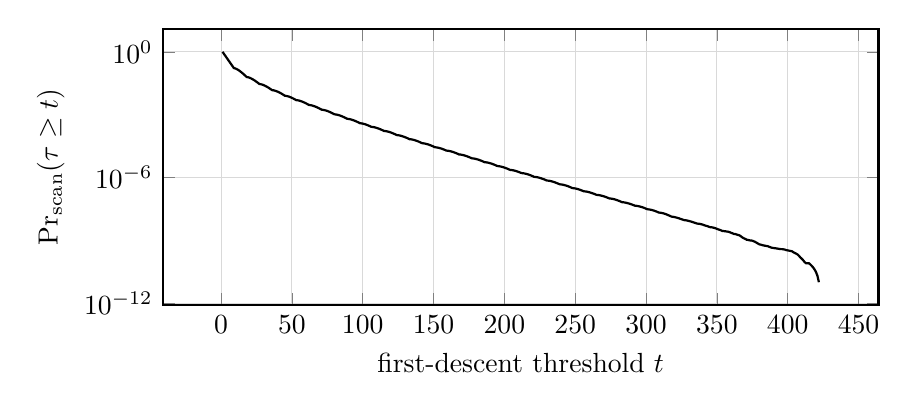
\begin{tikzpicture}
\begin{axis}[
width=0.88\textwidth,height=0.42\textwidth,
xlabel={first-descent threshold $t$},
ylabel={$\Pr_{\rm scan}(\tau\ge t)$},
ymode=log,
grid=both,
minor grid style={gray!15},
major grid style={gray!30},
mark=none,
line width=0.8pt
]
\addplot[black] coordinates {
(1,0.99999999999)
(2,0.79999999999)
(3,0.63999999999)
(4,0.51199999999)
(5,0.4096)
(6,0.32768)
(7,0.262144)
(8,0.2097152)
(9,0.16777216)
(10,0.1610612736)
(11,0.15032385526)
(12,0.13743895332)
(13,0.12369505606)
(14,0.10995116435)
(15,0.09675702375)
(16,0.08444248148)
(17,0.07318348768)
(18,0.06305040784)
(19,0.06124890195)
(20,0.05822255578)
(21,0.05441776195)
(22,0.05017497691)
(23,0.04574777542)
(24,0.04132038774)
(25,0.03702310619)
(26,0.03294309973)
(27,0.02913509718)
(28,0.02843401289)
(29,0.02723485758)
(30,0.02570007047)
(31,0.02395730524)
(32,0.02210549237)
(33,0.02021984606)
(34,0.01835637038)
(35,0.01655513586)
(36,0.0148439586)
(37,0.01452341644)
(38,0.01397001692)
(39,0.0132549023)
(40,0.01243469689)
(41,0.01155442292)
(42,0.01064891311)
(43,0.00974477888)
(44,0.00886184242)
(45,0.00801423434)
(46,0.0078536856)
(47,0.00757505094)
(48,0.00721279889)
(49,0.00679485756)
(50,0.00634350639)
(51,0.00587614978)
(52,0.00540654005)
(53,0.00494473963)
(54,0.00485546426)
(55,0.00469889742)
(56,0.00449335603)
(57,0.00425399966)
(58,0.00399305047)
(59,0.00372039076)
(60,0.00344381758)
(61,0.00316936489)
(62,0.00290172206)
(63,0.0028502251)
(64,0.00276006891)
(65,0.00264185475)
(66,0.00250421663)
(67,0.00235409636)
(68,0.00219720783)
(69,0.00203792128)
(70,0.00187967164)
(71,0.00172507823)
(72,0.00169526638)
(73,0.00164302582)
(74,0.00157441652)
(75,0.00149447562)
(76,0.00140720635)
(77,0.00131582227)
(78,0.00122282796)
(79,0.00113026227)
(80,0.00103966475)
(81,0.00102215379)
(82,0.0009914308)
(83,0.00095104991)
(84,0.00090386659)
(85,0.00085226378)
(86,0.00079815975)
(87,0.00074302613)
(88,0.00068803571)
(89,0.00063410153)
(90,0.0006236543)
(91,0.00060531178)
(92,0.00058117446)
(93,0.00055291096)
(94,0.00052196424)
(95,0.00048945257)
(96,0.00045629183)
(97,0.00042315489)
(98,0.00039059804)
(99,0.00038427646)
(100,0.00037317848)
(101,0.00035855197)
(102,0.00034142145)
(103,0.00032262933)
(104,0.00030287362)
(105,0.00028269742)
(106,0.00026252964)
(107,0.00025855471)
(108,0.00025151241)
(109,0.00024219308)
(110,0.0002312134)
(111,0.00021908565)
(112,0.00020626771)
(113,0.00019311052)
(114,0.00017987242)
(115,0.00016679397)
(116,0.00016424568)
(117,0.00015974505)
(118,0.00015380235)
(119,0.00014681091)
(120,0.00013910728)
(121,0.00013096423)
(122,0.00012261974)
(123,0.00011422969)
(124,0.00010595681)
(125,0.00010434356)
(126,0.00010150302)
(127,9.773963e-05)
(128,9.332014e-05)
(129,8.844985e-05)
(130,8.330739e-05)
(131,7.803138e-05)
(132,7.273219e-05)
(133,6.750083e-05)
(134,6.647553e-05)
(135,6.467407e-05)
(136,6.229382e-05)
(137,5.949542e-05)
(138,5.641679e-05)
(139,5.31649e-05)
(140,4.982701e-05)
(141,4.647469e-05)
(142,4.316225e-05)
(143,4.251549e-05)
(144,4.137579e-05)
(145,3.987001e-05)
(146,3.8099e-05)
(147,3.61461e-05)
(148,3.408237e-05)
(149,3.196439e-05)
(150,2.983825e-05)
(151,2.774176e-05)
(152,2.732983e-05)
(153,2.660126e-05)
(154,2.564134e-05)
(155,2.451191e-05)
(156,2.327095e-05)
(157,2.195275e-05)
(158,2.059527e-05)
(159,1.922807e-05)
(160,1.89568e-05)
(161,1.847552e-05)
(162,1.783711e-05)
(163,1.708327e-05)
(164,1.624721e-05)
(165,1.535777e-05)
(166,1.443819e-05)
(167,1.350918e-05)
(168,1.258888e-05)
(169,1.241027e-05)
(170,1.209055e-05)
(171,1.166718e-05)
(172,1.117033e-05)
(173,1.06242e-05)
(174,1.00436e-05)
(175,9.44208e-06)
(176,8.83359e-06)
(177,8.23215e-06)
(178,8.11481e-06)
(179,7.90585e-06)
(180,7.62852e-06)
(181,7.30196e-06)
(182,6.94088e-06)
(183,6.55895e-06)
(184,6.16794e-06)
(185,5.77558e-06)
(186,5.38352e-06)
(187,5.30682e-06)
(188,5.17145e-06)
(189,4.992e-06)
(190,4.78091e-06)
(191,4.54758e-06)
(192,4.29814e-06)
(193,4.04179e-06)
(194,3.7819e-06)
(195,3.5223e-06)
(196,3.47119e-06)
(197,3.38156e-06)
(198,3.26275e-06)
(199,3.12574e-06)
(200,2.97257e-06)
(201,2.80889e-06)
(202,2.64093e-06)
(203,2.47254e-06)
(204,2.30486e-06)
(205,2.27228e-06)
(206,2.21555e-06)
(207,2.13963e-06)
(208,2.05051e-06)
(209,1.95026e-06)
(210,1.84456e-06)
(211,1.73501e-06)
(212,1.62442e-06)
(213,1.6027e-06)
(214,1.56394e-06)
(215,1.51163e-06)
(216,1.44869e-06)
(217,1.37936e-06)
(218,1.3056e-06)
(219,1.22846e-06)
(220,1.15083e-06)
(221,1.07397e-06)
(222,1.05849e-06)
(223,1.03224e-06)
(224,9.9756e-07)
(225,9.5671e-07)
(226,9.1165e-07)
(227,8.6357e-07)
(228,8.1363e-07)
(229,7.6343e-07)
(230,7.1446e-07)
(231,7.052e-07)
(232,6.8789e-07)
(233,6.6455e-07)
(234,6.3682e-07)
(235,6.0643e-07)
(236,5.7409e-07)
(237,5.4131e-07)
(238,5.0766e-07)
(239,4.7316e-07)
(240,4.6654e-07)
(241,4.5484e-07)
(242,4.389e-07)
(243,4.2071e-07)
(244,4.0111e-07)
(245,3.7948e-07)
(246,3.5722e-07)
(247,3.3436e-07)
(248,3.1155e-07)
(249,3.0699e-07)
(250,2.9954e-07)
(251,2.891e-07)
(252,2.7704e-07)
(253,2.6348e-07)
(254,2.4889e-07)
(255,2.3366e-07)
(256,2.1919e-07)
(257,2.1636e-07)
(258,2.1142e-07)
(259,2.0461e-07)
(260,1.9653e-07)
(261,1.8772e-07)
(262,1.7824e-07)
(263,1.6815e-07)
(264,1.5805e-07)
(265,1.4809e-07)
(266,1.4616e-07)
(267,1.4287e-07)
(268,1.3829e-07)
(269,1.3292e-07)
(270,1.2691e-07)
(271,1.2072e-07)
(272,1.1409e-07)
(273,1.0732e-07)
(274,1.0026e-07)
(275,9.886e-08)
(276,9.638e-08)
(277,9.327e-08)
(278,8.96e-08)
(279,8.528e-08)
(280,8.051e-08)
(281,7.584e-08)
(282,7.112e-08)
(283,6.64e-08)
(284,6.549e-08)
(285,6.385e-08)
(286,6.19e-08)
(287,5.945e-08)
(288,5.668e-08)
(289,5.395e-08)
(290,5.122e-08)
(291,4.823e-08)
(292,4.526e-08)
(293,4.453e-08)
(294,4.343e-08)
(295,4.202e-08)
(296,4.049e-08)
(297,3.863e-08)
(298,3.666e-08)
(299,3.454e-08)
(300,3.238e-08)
(301,3.031e-08)
(302,2.989e-08)
(303,2.912e-08)
(304,2.811e-08)
(305,2.689e-08)
(306,2.555e-08)
(307,2.415e-08)
(308,2.27e-08)
(309,2.112e-08)
(310,2.083e-08)
(311,2.028e-08)
(312,1.956e-08)
(313,1.869e-08)
(314,1.77e-08)
(315,1.661e-08)
(316,1.552e-08)
(317,1.452e-08)
(318,1.351e-08)
(319,1.327e-08)
(320,1.287e-08)
(321,1.241e-08)
(322,1.193e-08)
(323,1.137e-08)
(324,1.072e-08)
(325,1.02e-08)
(326,9.7e-09)
(327,9.19e-09)
(328,9.09e-09)
(329,8.81e-09)
(330,8.47e-09)
(331,8.12e-09)
(332,7.78e-09)
(333,7.38e-09)
(334,7e-09)
(335,6.65e-09)
(336,6.29e-09)
(337,6.2e-09)
(338,6.07e-09)
(339,5.84e-09)
(340,5.61e-09)
(341,5.27e-09)
(342,5.01e-09)
(343,4.8e-09)
(344,4.56e-09)
(345,4.28e-09)
(346,4.21e-09)
(347,4.1e-09)
(348,3.96e-09)
(349,3.76e-09)
(350,3.53e-09)
(351,3.33e-09)
(352,3.16e-09)
(353,2.97e-09)
(354,2.77e-09)
(355,2.75e-09)
(356,2.7e-09)
(357,2.63e-09)
(358,2.57e-09)
(359,2.45e-09)
(360,2.29e-09)
(361,2.16e-09)
(362,2.02e-09)
(363,1.99e-09)
(364,1.89e-09)
(365,1.8e-09)
(366,1.72e-09)
(367,1.54e-09)
(368,1.37e-09)
(369,1.25e-09)
(370,1.17e-09)
(371,1.07e-09)
(372,1.04e-09)
(373,1e-09)
(374,9.8e-10)
(375,9.6e-10)
(376,9e-10)
(377,8.4e-10)
(378,7.7e-10)
(379,7e-10)
(380,6.4e-10)
(381,6.2e-10)
(382,5.9e-10)
(383,5.7e-10)
(384,5.5e-10)
(385,5.4e-10)
(386,5.2e-10)
(387,4.9e-10)
(388,4.6e-10)
(389,4.4e-10)
(390,4.3e-10)
(391,4.2e-10)
(392,4.1e-10)
(393,4e-10)
(394,3.9e-10)
(395,3.8e-10)
(396,3.8e-10)
(397,3.7e-10)
(398,3.6e-10)
(399,3.4e-10)
(400,3.3e-10)
(401,3.2e-10)
(402,3.1e-10)
(403,3e-10)
(404,2.7e-10)
(405,2.5e-10)
(406,2.3e-10)
(407,2.1e-10)
(408,1.8e-10)
(409,1.5e-10)
(410,1.3e-10)
(411,1.1e-10)
(412,9e-11)
(413,8e-11)
(414,8e-11)
(415,8e-11)
(416,7e-11)
(417,6e-11)
(418,5e-11)
(419,4e-11)
(420,3e-11)
(421,2e-11)
(422,1e-11)
};
\end{axis}
\end{tikzpicture}
\caption{Empirical survival function of the first-descent stopping time over all $10^{11}$ starts.}
\label{fig:tausurvival}
\end{figure}

\subsection{Historical first-descent records}

There are 22 strict historical records in $\tau(n)$ up to $10^{11}$. The terminal record is
\[
n=55{,}335{,}461{,}598,\qquad \tau=422.
\]

\begin{figure}[H]
\centering
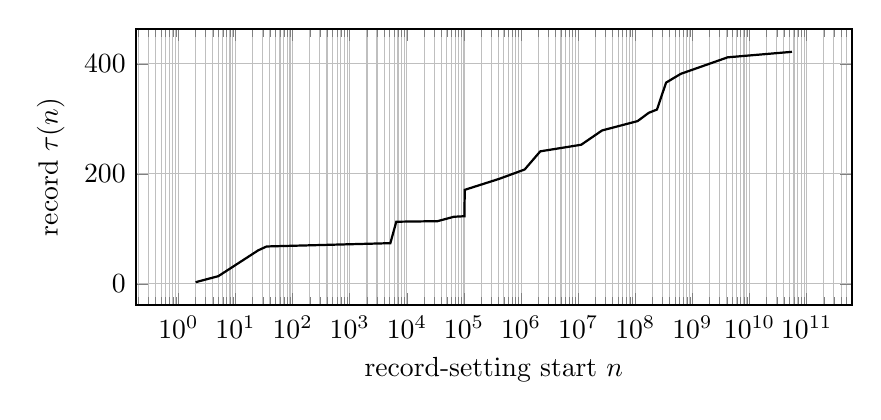
\begin{tikzpicture}
\begin{axis}[
width=0.88\textwidth,height=0.42\textwidth,
xmode=log,
xlabel={record-setting start $n$},
ylabel={record $\tau(n)$},
grid=both,
mark=*,
mark size=1.6pt,
line width=0.8pt
]
\addplot[black] coordinates {
(2,3)
(5,14)
(25,61)
(35,68)
(5140,74)
(6528,113)
(34430,114)
(66375,122)
(101765,123)
(103188,171)
(414675,191)
(1155414,208)
(2164875,241)
(11290165,253)
(26183590,279)
(109524730,296)
(171507948,311)
(239323602,317)
(345557052,366)
(626241035,382)
(4143683265,412)
(55335461598,422)
};
\end{axis}
\end{tikzpicture}
\caption{Historical staircase of first-descent records.}
\end{figure}

The complete record table, including first-lower values and pre-descent peaks recomputed from the deterministic map, appears in Appendix~\ref{app:tau-records}.

\section{Observed $5$-adic statistics}

The production run pooled all macro steps taken before first descent for all starts. This produced
\[
618{,}073{,}627{,}485
\]
growth operations. The observed brake-event fraction was
\[
\frac{123{,}614{,}478{,}358}{618{,}073{,}627{,}485}
=0.199999600146343,
\]
extremely close to the exact residue-density value $1/5$. The observed explicit divisions per growth step were
\[
0.249999815550697,
\]
close to the residue prediction $1/4$. Divisions per observed brake event were
\[
\frac{154{,}518{,}292{,}868}{123{,}614{,}478{,}358}
=1.250001576842,
\]
close to the conditional prediction $5/4$.

These comparisons are descriptive rather than iid significance tests: the pooled orbit states are deterministic and correlated.

\begin{table}[H]
\centering
\caption{Observed explicit valuation $e$ per growth step versus exact natural-residue prediction.}
\small
\begin{tabular}{r r r r r}
\toprule
$e$ & observed count & predicted probability & predicted count & relative error\\
\midrule
0 & 494{,}459{,}149{,}127 & 0.8 & 494{,}458{,}901{,}988 & +4.998e-07 \\
1 & 98{,}891{,}408{,}397 & 0.16 & 98{,}891{,}780{,}398 & -3.762e-06 \\
2 & 19{,}778{,}503{,}097 & 0.032 & 19{,}778{,}356{,}080 & +7.433e-06 \\
3 & 3{,}955{,}630{,}442 & 0.0064 & 3{,}955{,}671{,}216 & -1.031e-05 \\
4 & 791{,}143{,}958 & 0.00128 & 791{,}134{,}243 & +1.228e-05 \\
5 & 158{,}227{,}340 & 0.000256 & 158{,}226{,}849 & +3.105e-06 \\
6 & 31{,}656{,}239 & 5.12e-05 & 31{,}645{,}370 & +3.435e-04 \\
7 & 6{,}328{,}699 & 1.024e-05 & 6{,}329{,}074 & -5.924e-05 \\
8 & 1{,}263{,}921 & 2.048e-06 & 1{,}265{,}815 & -1.496e-03 \\
9 & 253{,}374 & 4.096e-07 & 253{,}163 & +8.336e-04 \\
10 & 50{,}520 & 8.192e-08 & 50{,}633 & -2.224e-03 \\
\bottomrule
\end{tabular}
\end{table}

\begin{figure}[H]
\centering
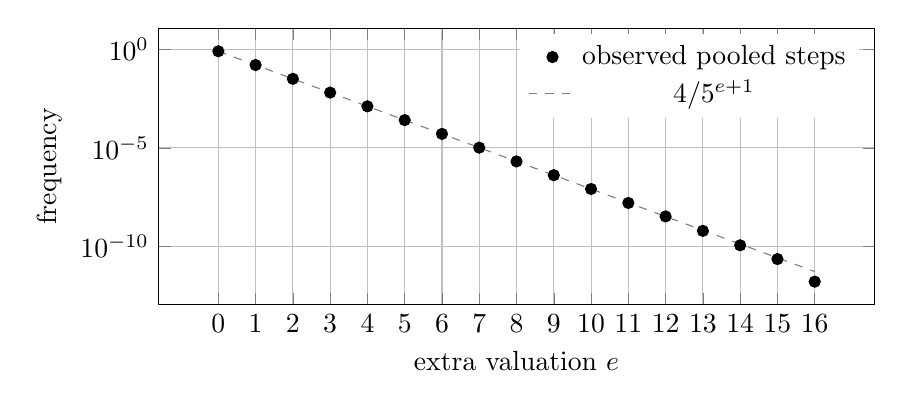
\begin{tikzpicture}
\begin{axis}[
width=0.88\textwidth,height=0.42\textwidth,
xlabel={extra valuation $e$},
ylabel={frequency},
ymode=log,
xtick={0,1,...,16},
grid=both,
legend style={at={(0.98,0.98)},anchor=north east,draw=none}
]
\addplot[only marks,mark=*,black] coordinates {
(0,0.800000399854)
(1,0.159999398129)
(2,0.032000237864)
(3,0.00639993403067)
(4,0.0012800157179)
(5,0.000256000794992)
(6,5.12175857249e-05)
(7,1.02393933644e-05)
(8,2.0449359814e-06)
(9,4.09941451524e-07)
(10,8.17378347068e-08)
(11,1.59495561073e-08)
(12,3.31675695069e-09)
(13,6.11577623103e-10)
(14,1.13255115389e-10)
(15,2.26510230779e-11)
(16,1.61793021985e-12)
};
\addlegendentry{observed pooled steps}
\addplot[mark=none,dashed,gray] coordinates {
(0,0.8)
(1,0.16)
(2,0.032)
(3,0.0064)
(4,0.00128)
(5,0.000256)
(6,5.12e-05)
(7,1.024e-05)
(8,2.048e-06)
(9,4.096e-07)
(10,8.192e-08)
(11,1.6384e-08)
(12,3.2768e-09)
(13,6.5536e-10)
(14,1.31072e-10)
(15,2.62144e-11)
(16,5.24288e-12)
};
\addlegendentry{$4/5^{e+1}$}
\end{axis}
\end{tikzpicture}
\caption{Observed pooled $5$-adic valuation frequencies and the exact one-step residue-density law.}
\end{figure}

The extreme valuation tail is also compatible in scale with the geometric law:
\begin{table}[H]
\centering
\caption{Counts with valuation at least $k$ compared with $M/5^k$, where $M$ is the total number of pooled macro steps.}
\begin{tabular}{lrr}
\toprule
Tail & observed & residue-model expected count\\
\midrule
$e\ge 10$ & 62{{,}}891 & 63{,}290.739 \\
$e\ge 11$ & 12{{,}}371 & 12{,}658.148 \\
$e\ge 12$ & 2{{,}}513 & 2{,}531.630 \\
$e\ge 13$ & 463 & 506.326 \\
$e\ge 14$ & 85 & 101.265 \\
$e\ge 15$ & 15 & 20.253 \\
$e\ge 16$ & 1 & 4.051 \\
$e\ge 17$ & 0 & 0.810 \\
\bottomrule
\end{tabular}
\end{table}
The scan saw one event with $e=16$ and none with $e\ge17$. Under a purely independent residue sample of the same size, the expected numbers with $e\ge16$ and $e\ge17$ would be about $4.05$ and $0.81$, respectively. The deterministic orbit sample is not independent, but the order of magnitude is consistent with the geometric tail.

\section{Extremal trajectories}

\subsection{The longest first descent}

For
\[
n_*=55{,}335{,}461{,}598
\]
the first strict descent occurs after
\[
\tau(n_*)=422
\]
macro steps. The first lower value is
\[
T^{422}(n_*)=40{,}450{,}990{,}568.
\]
The path uses $48$ explicit divisions by $5$ in total before first descent, so its elementary count is
\[
422+48=470.
\]
Its pre-descent peak is
\[
2{,}929{,}710{,}734{,}019{,}662,
\]
first reached at macro step 298. The largest individual explicit valuation on this record path is only $e=2$; its exceptional duration is therefore caused by the arrangement of many modest brakes rather than one extraordinarily deep $5$-adic collapse.

The first ten macro steps on this path are all non-brake growth steps. Near the peak,
\[
2{,}441{,}425{,}611{,}683{,}051
\mapsto
2{,}929{,}710{,}734{,}019{,}662,
\]
followed by a brake to
\[
703{,}130{,}576{,}164{,}719.
\]

\subsection{The largest peak}

The largest state seen before first descent over the entire scan is
\[
P_{\max}
=
8{,}669{,}800{,}813{,}122{,}806{,}007{,}604
\]
from
\[
n_P=37{,}266{,}730{,}278.
\]
It is reached at macro step 223, and
\[
\frac{P_{\max}}{n_P}
\approx 2.32642e+11.
\]
The trajectory's first descent occurs at step 350 with lower value 21{,}181{,}525{,}426.

Immediately after the peak, an $e=3$ brake sends the state to
\[
83{,}230{,}087{,}805{,}978{,}937{,}673,
\]
illustrating how a deep reduction can reverse a very long expansion. The peak exceeds the unsigned 64-bit ceiling by a factor of about 469.991, validating the use of 128-bit arithmetic.

\begin{figure}[H]
\centering
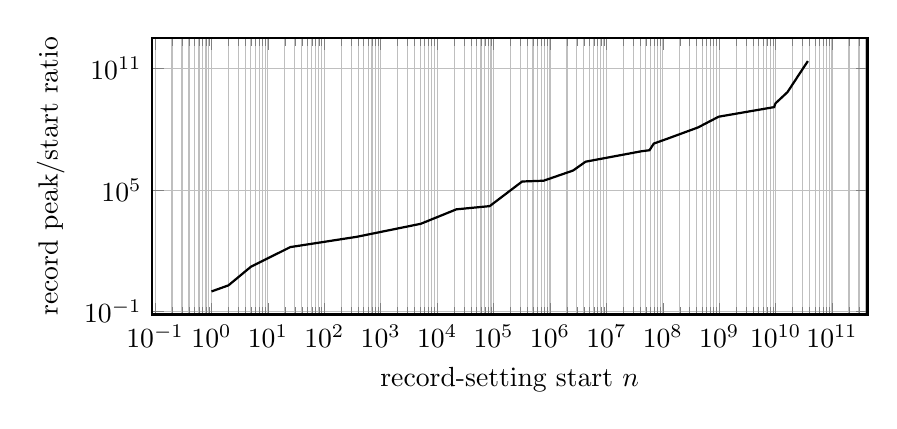
\begin{tikzpicture}
\begin{axis}[
width=0.88\textwidth,height=0.42\textwidth,
xmode=log,ymode=log,
xlabel={record-setting start $n$},
ylabel={record peak/start ratio},
grid=both,
mark=*,
mark size=1.5pt,
line width=0.8pt
]
\addplot[black] coordinates {
(1,1)
(2,2)
(5,16.6)
(25,154.64)
(375,496.298666667)
(5140,2185.14669261)
(21924,11271.0321109)
(85400,16228.5979625)
(321605,266263.949979)
(771455,290742.030599)
(2566640,924520.260624)
(4281725,2528168.90261)
(41651352,8243105.58988)
(57997600,9288587.5433)
(69399738,19876314.523)
(113912244,32459601.8008)
(419608488,123068897.362)
(978453590,419436904.994)
(9411506300,1244423202.55)
(9935817390,1908327954.97)
(16192618210,6794159216.64)
(37266730278,232641842964)
};
\end{axis}
\end{tikzpicture}
\caption{Historical record staircase of the pre-descent peak-to-start ratio.}
\end{figure}

\subsection{The deepest observed $5$-adic brake}

The first starting value whose pre-descent path reaches $e=16$ is
\[
n_V=88{,}717{,}666{,}380.
\]
After eight growth steps the orbit reaches
\[
381{,}469{,}726{,}562.
\]
Then
\[
G(381{,}469{,}726{,}562)
=
457{,}763{,}671{,}875
=
3\cdot5^{16},
\]
so the next reduced state is exactly
\[
3.
\]
Thus a single brake removes sixteen explicit factors of $5$.

\section{Relation to the companion $6k\pm1(2)/5$ domain}

A companion work studies the related $6k\pm1(2)/5$ Collatz-type domain and its finite computational behavior \cite{BanazadehCompanion}. It is cited here as part of the same broader sequence-computation program and reproducibility framework. The present floor-$6/5$ map is nevertheless treated as a distinct dynamical system: its floor-affine rule, complete $5$-adic reduction, residue classes, stopping-time distribution, and cycle constraints are developed directly in the preceding sections. No numerical statistic from the companion domain is used in the proofs or finite-range conclusions of the present paper.

\section{What is exact, what is computational, and what is heuristic}

The conclusions separate into three categories.

\paragraph{Exact algebra.}
The residue form \eqref{eq:affine}, closure of $\D$, the exact four-cycle, absence of fixed points, valuation-density law \eqref{eq:geom}, inverse branches, cycle identity \eqref{eq:cycleidentity}, and cycle-balance condition \eqref{eq:cyclethreshold} are exact mathematical statements.

\paragraph{Exhaustive finite computation.}
Under the supplied implementation and its checked 128-bit arithmetic, every one of the $\Nscan$ starting values through $10^{11}$ obtained a strict first descent. The maximum first-descent time is 422. Strong induction therefore establishes entry into $\Cyc$ for every start in the tested interval. The record statistics, histograms, and extremal states are direct outputs of the completed scan or deterministic recomputations from its recorded extremal starts.

\paragraph{Probabilistic interpretation.}
Treating successive residue states as sufficiently mixing converts the exact one-step valuation density into an approximate stochastic process. The negative logarithmic drift and critical first moment explain the observed combination of frequent descent and rare extreme excursions. This interpretation does not prove that every positive integer eventually enters $\Cyc$, nor does it rule out a cycle whose minimum state exceeds $10^{11}$.

\section{Reproducibility archive}

The accompanying compact archive is designed to permit both direct inspection of the completed computation and independent regeneration.

The essential files are:
\begin{itemize}
\item \texttt{firstlower\_certificate.cpp}: production C++ scanner using unsigned 128-bit arithmetic;
\item \texttt{aggregate\_certificate.py}: deterministic aggregation of chunk certificates;
\item \texttt{certificate\_chunks/}: the 4000 production JSON chunk certificates, with redundant \texttt{.done} sentinels omitted;
\item \texttt{results/summary.json}: final headline statistics;
\item \texttt{results/manifest.csv}: per-chunk result digests and JSON SHA-256 values;
\item exact histograms and record-staircase CSV files;
\item the production terminal log;
\item this \LaTeX{} source.
\end{itemize}

A complete regeneration uses the same finite interval and chunk size:
\begin{Verbatim}[fontsize=\small]
clang++ -O3 -std=c++17 -pthread firstlower_certificate.cpp \
  -o firstlower_certificate

./firstlower_certificate \
  --begin 1 \
  --end 100000000000 \
  --chunk 25000000 \
  --threads 4 \
  --out certificate_1e11

python3 aggregate_certificate.py certificate_1e11 \
  --out zenodo_certificate_1e11
\end{Verbatim}
Independent reproduction can compare each canonical result digest in \texttt{manifest.csv}. The public repository for the broader sequence-computation program is
\[
\text{\url{https://github.com/FarhadBanazadeh/sequence-computations}}.
\]

\section{Conclusion}

The map
\[
T(n)=5^{-\nuFive(\lfloor6n/5\rfloor+1)}
\left(\left\lfloor\frac{6n}{5}\right\rfloor+1\right)
\]
has a compact definition but a rich arithmetic structure. Every non-brake step grows, every brake step contracts, and the brake depth has an exact geometric $5$-adic density. In the natural residue model, the approximate multiplier is critical in arithmetic mean,
\[
\mathbb E[M]=1,
\]
while its logarithmic mean is strictly negative,
\[
\mathbb E[\log M]\approx -0.220037921315.
\]
This offers a precise mechanism for the observed combination of typical descent and rare large excursions.

The exact cycle identity shows that any periodic orbit must have total $5$-adic exponent exceeding the $6^L$ growth threshold, and a large hypothetical cycle would need a valuation profile biased below the natural mean. The inverse branches give a complementary exact description of the predecessor structure of the four-cycle.

Computationally, every integer through $10^{11}$ has been exhaustively certified to descend below itself, with maximum first-descent time 422. By strong induction, every start in this range enters the exact cycle
\[
1\mapsto2\mapsto3\mapsto4\mapsto1.
\]
The largest observed pre-descent state exceeds $8.66\times10^{21}$, showing that finite convergence can coexist with extremely large transients.

The global problem remains open: the present work does not prove convergence for all positive integers or absolute uniqueness of the four-cycle. It does, however, combine exact residue algebra, a critical multiplicative model, and a complete $10^{11}$ first-descent certificate into a single reproducible finite result.

\appendix

\section{Complete historical first-descent records}
\label{app:tau-records}

The following table lists all 22 strict historical records of $\tau(n)$ through $10^{11}$. The first-lower value, elementary count, and peak data were recomputed deterministically from each record-setting start using the same map.

\begin{longtable}{r r r r r r}
\caption{Complete first-descent record staircase.}\\
\toprule
$n$ & $\tau$ & first lower & elementary & pre-descent peak & peak step\\
\midrule
\endfirsthead
\toprule
$n$ & $\tau$ & first lower & elementary & pre-descent peak & peak step\\
\midrule
\endhead
2 & 3 & 1 & 4 & 4 & 2 \\
5 & 14 & 4 & 16 & 83 & 13 \\
25 & 61 & 1 & 70 & 3{,}866 & 27 \\
35 & 68 & 1 & 78 & 3{,}866 & 34 \\
5{,}140 & 74 & 381 & 84 & 11{,}231{,}654 & 51 \\
6{,}528 & 113 & 4{,}743 & 126 & 2{,}783{,}337 & 95 \\
34{,}430 & 114 & 29{,}998 & 127 & 21{,}801{,}416 & 106 \\
66{,}375 & 122 & 49{,}724 & 136 & 536{,}079{,}016 & 67 \\
101{,}765 & 123 & 91{,}481 & 137 & 101{,}304{,}629 & 82 \\
103{,}188 & 171 & 37{,}519 & 191 & 213{,}001{,}433 & 86 \\
414{,}675 & 191 & 231{,}206 & 213 & 70{,}541{,}954 & 37 \\
1{,}155{,}414 & 208 & 114{,}338 & 233 & 230{,}028{,}116 & 82 \\
2{,}164{,}875 & 241 & 702{,}999 & 269 & 41{,}380{,}285{,}491 & 160 \\
11{,}290{,}165 & 253 & 6{,}537{,}711 & 282 & 11{,}187{,}289{,}322{,}954 & 164 \\
26{,}183{,}590 & 279 & 13{,}885{,}348 & 311 & 11{,}824{,}755{,}492{,}887 & 195 \\
109{,}524{,}730 & 296 & 10{,}308{,}866 & 331 & 245{,}431{,}223{,}308 & 263 \\
171{,}507{,}948 & 311 & 9{,}948{,}592 & 348 & 57{,}280{,}540{,}172{,}679 & 211 \\
239{,}323{,}602 & 317 & 207{,}262{,}333 & 353 & 57{,}280{,}540{,}172{,}679 & 218 \\
345{,}557{,}052 & 366 & 145{,}249{,}833 & 408 & 14{,}585{,}673{,}548{,}633 & 182 \\
626{,}241{,}035 & 382 & 194{,}669{,}236 & 426 & 2{,}023{,}256{,}411{,}512{,}679 & 144 \\
4{,}143{,}683{,}265 & 412 & 2{,}446{,}074{,}722 & 459 & 1{,}660{,}697{,}930{,}418{,}566 & 212 \\
55{,}335{,}461{,}598 & 422 & 40{,}450{,}990{,}568 & 470 & 2{,}929{,}710{,}734{,}019{,}662 & 298 \\
\bottomrule
\end{longtable}

\section{Historical elementary-step records}

\begin{longtable}{r r}
\caption{Historical records of the elementary step count before first descent.}\\
\toprule
$n$ & elementary steps\\
\midrule
\endfirsthead
\toprule
$n$ & elementary steps\\
\midrule
\endhead
2 & 4 \\
5 & 16 \\
25 & 70 \\
35 & 78 \\
5{,}140 & 84 \\
6{,}528 & 126 \\
34{,}430 & 127 \\
66{,}375 & 136 \\
87{,}515 & 137 \\
103{,}188 & 191 \\
414{,}675 & 213 \\
1{,}155{,}414 & 233 \\
2{,}164{,}875 & 269 \\
11{,}290{,}165 & 282 \\
26{,}183{,}590 & 311 \\
109{,}524{,}730 & 331 \\
171{,}507{,}948 & 348 \\
239{,}323{,}602 & 353 \\
345{,}557{,}052 & 408 \\
626{,}241{,}035 & 426 \\
4{,}143{,}683{,}265 & 459 \\
55{,}335{,}461{,}598 & 470 \\
\bottomrule
\end{longtable}

\section{Historical maximum-valuation records}

\begin{longtable}{r r}
\caption{Historical records of the largest explicit valuation $e$ encountered before first descent.}\\
\toprule
$n$ & record $e$\\
\midrule
\endfirsthead
\toprule
$n$ & record $e$\\
\midrule
\endhead
2 & 1 \\
5 & 2 \\
25 & 3 \\
300 & 4 \\
2{,}604 & 5 \\
13{,}020 & 6 \\
45{,}210 & 7 \\
227{,}115 & 8 \\
1{,}356{,}336 & 9 \\
8{,}138{,}020 & 10 \\
40{,}690{,}104 & 11 \\
203{,}450{,}520 & 12 \\
408{,}811{,}005 & 13 \\
5{,}086{,}263{,}020 & 14 \\
17{,}660{,}635{,}488 & 15 \\
88{,}717{,}666{,}380 & 16 \\
\bottomrule
\end{longtable}

\section{Historical peak records}

\begin{longtable}{r r}
\caption{Historical records of the largest pre-descent state.}\\
\toprule
$n$ & record peak\\
\midrule
\endfirsthead
\toprule
$n$ & record peak\\
\midrule
\endhead
1 & 1 \\
2 & 4 \\
5 & 83 \\
25 & 3{,}866 \\
255 & 7{,}091 \\
375 & 186{,}112 \\
2{,}390 & 190{,}216 \\
3{,}936 & 224{,}379 \\
3{,}942 & 376{,}304 \\
4{,}488 & 1{,}841{,}979 \\
5{,}140 & 11{,}231{,}654 \\
9{,}185 & 14{,}380{,}587 \\
18{,}460 & 27{,}135{,}933 \\
21{,}924 & 247{,}106{,}108 \\
43{,}368 & 433{,}754{,}637 \\
66{,}375 & 536{,}079{,}016 \\
85{,}400 & 1{,}385{,}922{,}266 \\
133{,}050 & 1{,}743{,}613{,}383 \\
285{,}935 & 2{,}685{,}317{,}283 \\
321{,}605 & 85{,}631{,}817{,}633 \\
771{,}455 & 224{,}294{,}393{,}216 \\
2{,}566{,}640 & 2{,}372{,}910{,}681{,}729 \\
3{,}049{,}380 & 2{,}819{,}212{,}783{,}283 \\
4{,}281{,}725 & 10{,}824{,}923{,}994{,}533 \\
11{,}290{,}165 & 11{,}187{,}289{,}322{,}954 \\
13{,}240{,}296 & 17{,}626{,}908{,}865{,}258 \\
20{,}631{,}036 & 24{,}374{,}775{,}827{,}804 \\
28{,}654{,}488 & 41{,}923{,}225{,}824{,}033 \\
41{,}651{,}352 & 343{,}336{,}492{,}497{,}254 \\
57{,}997{,}600 & 538{,}715{,}784{,}901{,}533 \\
69{,}399{,}738 & 1{,}379{,}411{,}020{,}304{,}104 \\
113{,}912{,}244 & 3{,}697{,}546{,}080{,}480{,}512 \\
325{,}104{,}490 & 3{,}739{,}513{,}277{,}224{,}208 \\
340{,}154{,}598 & 8{,}165{,}437{,}450{,}887{,}116 \\
419{,}608{,}488 & 51{,}640{,}753{,}941{,}727{,}516 \\
978{,}453{,}590 & 410{,}399{,}545{,}469{,}610{,}633 \\
1{,}817{,}298{,}498 & 574{,}304{,}230{,}615{,}862{,}066 \\
6{,}015{,}661{,}296 & 1{,}487{,}631{,}812{,}946{,}202{,}666 \\
7{,}013{,}390{,}365 & 1{,}691{,}472{,}330{,}963{,}023{,}741 \\
9{,}411{,}506{,}300 & 11{,}711{,}896{,}810{,}632{,}293{,}579 \\
9{,}935{,}817{,}390 & 18{,}960{,}798{,}080{,}788{,}942{,}641 \\
16{,}192{,}618{,}210 & 110{,}015{,}226{,}253{,}048{,}021{,}408 \\
37{,}266{,}730{,}278 & 8{,}669{,}800{,}813{,}122{,}806{,}007{,}604 \\
\bottomrule
\end{longtable}

\section{Historical peak-ratio records}

\begin{longtable}{r r r}
\caption{Historical records of the pre-descent peak/start ratio.}\\
\toprule
$n$ & peak & peak$/n$ (approx.)\\
\midrule
\endfirsthead
\toprule
$n$ & peak & peak$/n$ (approx.)\\
\midrule
\endhead
1 & 1 & 1 \\
2 & 4 & 2 \\
5 & 83 & 16.6 \\
25 & 3{,}866 & 154.64 \\
375 & 186{,}112 & 496.299 \\
5{,}140 & 11{,}231{,}654 & 2185.15 \\
21{,}924 & 247{,}106{,}108 & 11271 \\
85{,}400 & 1{,}385{,}922{,}266 & 16228.6 \\
321{,}605 & 85{,}631{,}817{,}633 & 266264 \\
771{,}455 & 224{,}294{,}393{,}216 & 290742 \\
2{,}566{,}640 & 2{,}372{,}910{,}681{,}729 & 924520 \\
4{,}281{,}725 & 10{,}824{,}923{,}994{,}533 & 2.52817e+06 \\
41{,}651{,}352 & 343{,}336{,}492{,}497{,}254 & 8.24311e+06 \\
57{,}997{,}600 & 538{,}715{,}784{,}901{,}533 & 9.28859e+06 \\
69{,}399{,}738 & 1{,}379{,}411{,}020{,}304{,}104 & 1.98763e+07 \\
113{,}912{,}244 & 3{,}697{,}546{,}080{,}480{,}512 & 3.24596e+07 \\
419{,}608{,}488 & 51{,}640{,}753{,}941{,}727{,}516 & 1.23069e+08 \\
978{,}453{,}590 & 410{,}399{,}545{,}469{,}610{,}633 & 4.19437e+08 \\
9{,}411{,}506{,}300 & 11{,}711{,}896{,}810{,}632{,}293{,}579 & 1.24442e+09 \\
9{,}935{,}817{,}390 & 18{,}960{,}798{,}080{,}788{,}942{,}641 & 1.90833e+09 \\
16{,}192{,}618{,}210 & 110{,}015{,}226{,}253{,}048{,}021{,}408 & 6.79416e+09 \\
37{,}266{,}730{,}278 & 8{,}669{,}800{,}813{,}122{,}806{,}007{,}604 & 2.32642e+11 \\
\bottomrule
\end{longtable}

\begin{thebibliography}{9}

\bibitem{Lagarias1985}
J. C. Lagarias,
``The $3x+1$ problem and its generalizations,''
\emph{American Mathematical Monthly} 92 (1985), 3--23.

\bibitem{Lagarias2010}
J. C. Lagarias (ed.),
\emph{The Ultimate Challenge: The $3x+1$ Problem},
American Mathematical Society, 2010.

\bibitem{BanazadehCompanion}
F. Banazadeh,
``The $6k\pm1(2)/5$ Collatz-Type Domain,''
Zenodo, 16 September 2026,
\url{https://doi.org/10.5281/zenodo.22786203}.

\bibitem{Repository}
F. Banazadeh,
\emph{Sequence Computations: research articles, source code, computational packages, and reproducibility materials},
2026,
\url{https://github.com/FarhadBanazadeh/sequence-computations}.

\end{thebibliography}

\end{document}
